\section{Arquitetura}

\subsection{Representação da Arquitetura}

A forma como está sendo utilizado o framework Ionic pode ser representado com diagrama de pacotes representado na Figura \ref{img:pacotes}:

\begin{figure}[H]
    \centering
    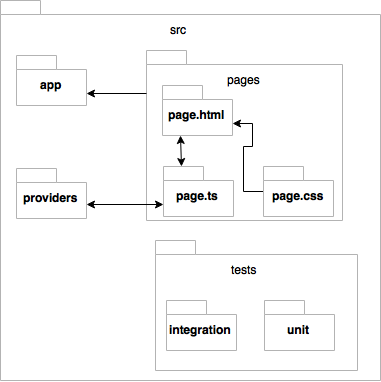
\includegraphics[scale=0.5]{figuras/ionic_arch.png}
    \caption[Diagrama de pacotes do aplicativo]{Diagrama de pacotes. Fonte: autores}
    \label{img:pacotes}
\end{figure}

A arquitetura da API é baseada na arquitetura MVC e está definida como ilustra a Figura \ref{img:arquitetura}:

\begin{figure}[H]
    \centering
    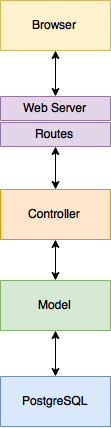
\includegraphics[scale=0.5]{figuras/api_arch.png}
    \caption[Arquitetura da API]{Arquitetura da API. Fonte: autores}
    \label{img:arquitetura}
\end{figure}


\subsection{Modelo de Dados}

Utilizando a ferramenta MySQL Workbench, foi criado um modelo de dados da aplicação. O dicionário de dados pode ser encontrado no Anexo \ref{chap:dicionario}. O modelo da aplicação é representado pela Figura \ref{img:modelo_de_dados}:

\begin{figure}[H]
    \centering
    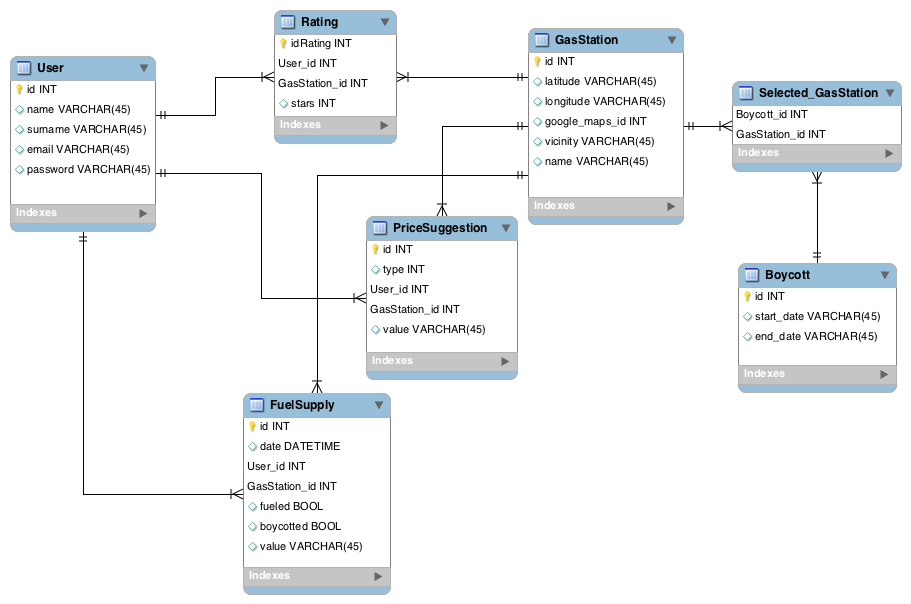
\includegraphics[scale=0.5]{figuras/db_model.png}
    \caption[Modelo de dados]{Modelo de dados Fonte: autores}
    \label{img:modelo_de_dados}
\end{figure}
